\subsection{Stubfilter}

Im Kapitel \ref{sec:Protototypfilter} wurde gezeigt, wie durch die Entnormierung eines Prototypfilter ein konkretes LC-Filter dimensioniert werden kann. Solche LC-Filter  können in einem weiten Frequenzbereich  eingesetzt  werden.  Jedoch
wird  bei realen konzentrierten Elementen (R,L,C) zu höheren Frequenzen hin der Einfluss der parasitären Eigenschaften immer deutlicher, so dass hohe Anforderungen an die Bauteilgüte  gestellt  werden  müssen. Im GHZ-Bereich wird es daher  zunehmend attraktiv,  statt  konzentrierten  Kapazitäten  und  Induktivitäten  verteilte
Strukturen  in  Form  von  Leitungen  zu  verwenden.  Man  spricht   dann  von sogenannten Leitungsfiltern.
%Quelle direktes Zitat: 
%https://books.google.ch/books?id=MTVQAgAAQBAJ&pg=PA203&lpg=PA203&dq=leitungsfilter+hochfrequenztechnik&source=bl&ots=Ljf0GRJkZt&sig=n-0G9H5VZ9iuPc2qepAATnjA47M&hl=de&sa=X&ved=0ahUKEwj38u-T79DUAhUSL1AKHUsyDNMQ6AEINTAB#v=onepage&q=leitungsfilter%20hochfrequenztechnik&f=false%

Es gibt verschiedene Arten um  Leitungsfilter zu realisieren. Eine Möglichkeit der  Realisierung  ist das Stubfilter.  Dieses  Filter  verwendet  gleichlange kurzgeschlossenen Leitungen (TLSC) und  leerlaufende  Leitungen(TLOC), welche an einem Ende verbunden und am anderen Ende entweder kurzgeschlossen
oder offen gelassen werden. Diese sogenannten Stubs oder Stichleitungen werden mit gleichlangen Verbindunsleitungen (TLIN) verbunden. 

In Abb. \ref{fig:Stubfilter} ist ein solches Stubfilter zu sehen, welches aus 8 kurgeschlossenen Stubs (TLSC) besteht.

\begin{figure}[h!]
\centering
 	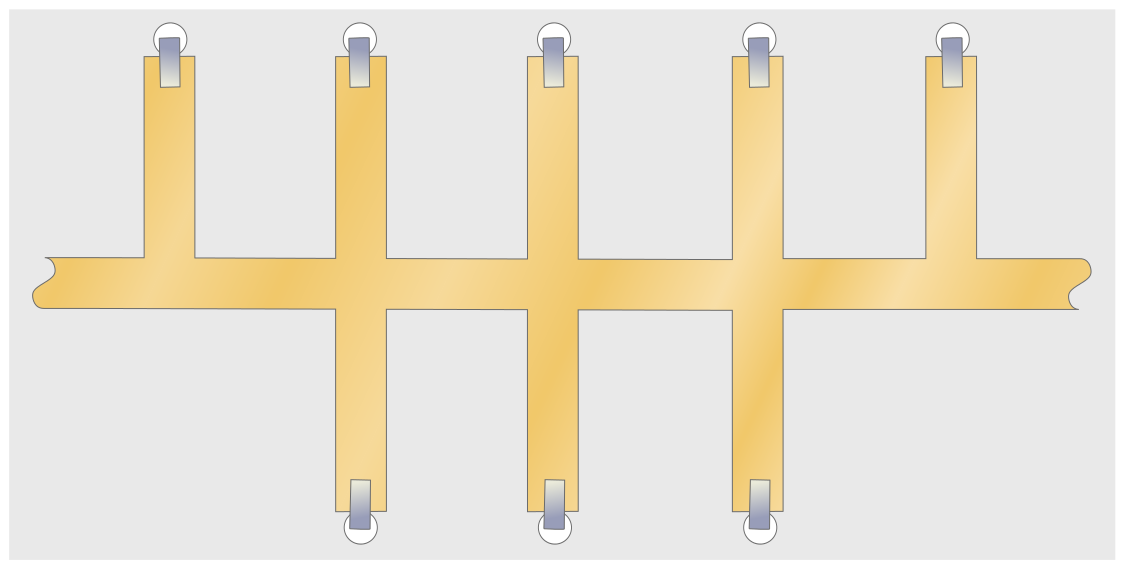
\includegraphics[width=\imagewidth]{images/Stripline_Stub_Filter}
 	\caption{Stubfilter}
 	\label{fig:Stubfilter}
\end{figure}

%Quelle: Wikipedia https://en.wikipedia.org/wiki/File:Stripline_stub_filter.svg

Stubs verhalten sich bei  hohen  Frequenzen  wie  reaktive Elemente(L,C) und ermöglichen so die Realisierung  eines  Mikrowellenfilters. Für Stubfilter existiert eine geschlossene Thoerie zur Filtersynthese. Dadurch muss ein herrkömmliches Prototypfilter nur entnormiert und transformiert werden, um das gewünschte Stubfilter mit den gewünschten Eigenschaften zu erhalten.

